\PassOptionsToPackage{unicode=true}{hyperref} % options for packages loaded elsewhere
\PassOptionsToPackage{hyphens}{url}
%
\documentclass[
  ignorenonframetext,
]{beamer}
\usepackage{pgfpages}
\setbeamertemplate{caption}[numbered]
\setbeamertemplate{caption label separator}{: }
\setbeamercolor{caption name}{fg=normal text.fg}
\beamertemplatenavigationsymbolsempty
% Prevent slide breaks in the middle of a paragraph:
\widowpenalties 1 10000
\raggedbottom
\setbeamertemplate{part page}{
  \centering
  \begin{beamercolorbox}[sep=16pt,center]{part title}
    \usebeamerfont{part title}\insertpart\par
  \end{beamercolorbox}
}
\setbeamertemplate{section page}{
  \centering
  \begin{beamercolorbox}[sep=12pt,center]{part title}
    \usebeamerfont{section title}\insertsection\par
  \end{beamercolorbox}
}
\setbeamertemplate{subsection page}{
  \centering
  \begin{beamercolorbox}[sep=8pt,center]{part title}
    \usebeamerfont{subsection title}\insertsubsection\par
  \end{beamercolorbox}
}
\AtBeginPart{
  \frame{\partpage}
}
\AtBeginSection{
  \ifbibliography
  \else
    \frame{\sectionpage}
  \fi
}
\AtBeginSubsection{
  \frame{\subsectionpage}
}
\usepackage{lmodern}
\usepackage{amssymb,amsmath}
\usepackage{ifxetex,ifluatex}
\ifnum 0\ifxetex 1\fi\ifluatex 1\fi=0 % if pdftex
  \usepackage[T1]{fontenc}
  \usepackage[utf8]{inputenc}
  \usepackage{textcomp} % provides euro and other symbols
\else % if luatex or xelatex
  \usepackage{unicode-math}
  \defaultfontfeatures{Scale=MatchLowercase}
  \defaultfontfeatures[\rmfamily]{Ligatures=TeX,Scale=1}
\fi
% use upquote if available, for straight quotes in verbatim environments
\IfFileExists{upquote.sty}{\usepackage{upquote}}{}
\IfFileExists{microtype.sty}{% use microtype if available
  \usepackage[]{microtype}
  \UseMicrotypeSet[protrusion]{basicmath} % disable protrusion for tt fonts
}{}
\makeatletter
\@ifundefined{KOMAClassName}{% if non-KOMA class
  \IfFileExists{parskip.sty}{%
    \usepackage{parskip}
  }{% else
    \setlength{\parindent}{0pt}
    \setlength{\parskip}{6pt plus 2pt minus 1pt}}
}{% if KOMA class
  \KOMAoptions{parskip=half}}
\makeatother
\usepackage{xcolor}
\IfFileExists{xurl.sty}{\usepackage{xurl}}{} % add URL line breaks if available
\IfFileExists{bookmark.sty}{\usepackage{bookmark}}{\usepackage{hyperref}}
\hypersetup{
  pdftitle={Github: The beginning},
  pdfauthor={Brock Kamrath},
  pdfborder={0 0 0},
  breaklinks=true}
\urlstyle{same}  % don't use monospace font for urls
\newif\ifbibliography
\usepackage{color}
\usepackage{fancyvrb}
\newcommand{\VerbBar}{|}
\newcommand{\VERB}{\Verb[commandchars=\\\{\}]}
\DefineVerbatimEnvironment{Highlighting}{Verbatim}{commandchars=\\\{\}}
% Add ',fontsize=\small' for more characters per line
\usepackage{framed}
\definecolor{shadecolor}{RGB}{248,248,248}
\newenvironment{Shaded}{\begin{snugshade}}{\end{snugshade}}
\newcommand{\AlertTok}[1]{\textcolor[rgb]{0.94,0.16,0.16}{#1}}
\newcommand{\AnnotationTok}[1]{\textcolor[rgb]{0.56,0.35,0.01}{\textbf{\textit{#1}}}}
\newcommand{\AttributeTok}[1]{\textcolor[rgb]{0.77,0.63,0.00}{#1}}
\newcommand{\BaseNTok}[1]{\textcolor[rgb]{0.00,0.00,0.81}{#1}}
\newcommand{\BuiltInTok}[1]{#1}
\newcommand{\CharTok}[1]{\textcolor[rgb]{0.31,0.60,0.02}{#1}}
\newcommand{\CommentTok}[1]{\textcolor[rgb]{0.56,0.35,0.01}{\textit{#1}}}
\newcommand{\CommentVarTok}[1]{\textcolor[rgb]{0.56,0.35,0.01}{\textbf{\textit{#1}}}}
\newcommand{\ConstantTok}[1]{\textcolor[rgb]{0.00,0.00,0.00}{#1}}
\newcommand{\ControlFlowTok}[1]{\textcolor[rgb]{0.13,0.29,0.53}{\textbf{#1}}}
\newcommand{\DataTypeTok}[1]{\textcolor[rgb]{0.13,0.29,0.53}{#1}}
\newcommand{\DecValTok}[1]{\textcolor[rgb]{0.00,0.00,0.81}{#1}}
\newcommand{\DocumentationTok}[1]{\textcolor[rgb]{0.56,0.35,0.01}{\textbf{\textit{#1}}}}
\newcommand{\ErrorTok}[1]{\textcolor[rgb]{0.64,0.00,0.00}{\textbf{#1}}}
\newcommand{\ExtensionTok}[1]{#1}
\newcommand{\FloatTok}[1]{\textcolor[rgb]{0.00,0.00,0.81}{#1}}
\newcommand{\FunctionTok}[1]{\textcolor[rgb]{0.00,0.00,0.00}{#1}}
\newcommand{\ImportTok}[1]{#1}
\newcommand{\InformationTok}[1]{\textcolor[rgb]{0.56,0.35,0.01}{\textbf{\textit{#1}}}}
\newcommand{\KeywordTok}[1]{\textcolor[rgb]{0.13,0.29,0.53}{\textbf{#1}}}
\newcommand{\NormalTok}[1]{#1}
\newcommand{\OperatorTok}[1]{\textcolor[rgb]{0.81,0.36,0.00}{\textbf{#1}}}
\newcommand{\OtherTok}[1]{\textcolor[rgb]{0.56,0.35,0.01}{#1}}
\newcommand{\PreprocessorTok}[1]{\textcolor[rgb]{0.56,0.35,0.01}{\textit{#1}}}
\newcommand{\RegionMarkerTok}[1]{#1}
\newcommand{\SpecialCharTok}[1]{\textcolor[rgb]{0.00,0.00,0.00}{#1}}
\newcommand{\SpecialStringTok}[1]{\textcolor[rgb]{0.31,0.60,0.02}{#1}}
\newcommand{\StringTok}[1]{\textcolor[rgb]{0.31,0.60,0.02}{#1}}
\newcommand{\VariableTok}[1]{\textcolor[rgb]{0.00,0.00,0.00}{#1}}
\newcommand{\VerbatimStringTok}[1]{\textcolor[rgb]{0.31,0.60,0.02}{#1}}
\newcommand{\WarningTok}[1]{\textcolor[rgb]{0.56,0.35,0.01}{\textbf{\textit{#1}}}}
\usepackage{graphicx,grffile}
\makeatletter
\def\maxwidth{\ifdim\Gin@nat@width>\linewidth\linewidth\else\Gin@nat@width\fi}
\def\maxheight{\ifdim\Gin@nat@height>\textheight\textheight\else\Gin@nat@height\fi}
\makeatother
% Scale images if necessary, so that they will not overflow the page
% margins by default, and it is still possible to overwrite the defaults
% using explicit options in \includegraphics[width, height, ...]{}
\setkeys{Gin}{width=\maxwidth,height=\maxheight,keepaspectratio}
\setlength{\emergencystretch}{3em}  % prevent overfull lines
\providecommand{\tightlist}{%
  \setlength{\itemsep}{0pt}\setlength{\parskip}{0pt}}
\setcounter{secnumdepth}{-2}

% set default figure placement to htbp
\makeatletter
\def\fps@figure{htbp}
\makeatother


\title{Github: The beginning}
\author{Brock Kamrath}
\date{1/18/2021}

\begin{document}
\frame{\titlepage}

\begin{frame}{Introduction}
\protect\hypertarget{introduction}{}

Welcome to Version Control week!

\includegraphics[width=10.67in]{pres_figs/github_logo2}

\begin{itemize}
\tightlist
\item
  In our lectures and excercises on version control with GitHub, we will
  largely utilize

  \begin{itemize}
  \tightlist
  \item
    \emph{Happy Git and GitHub for the useR} by Jennifer Bryan @
    happygitwithr.com
  \item
    \emph{Introduction to Github} by Lise Montefiore for REEU P4 program
  \end{itemize}
\end{itemize}

\end{frame}

\begin{frame}{Today's Schedule}
\protect\hypertarget{todays-schedule}{}

\begin{itemize}
\tightlist
\item
  Discussion of readings
\item
  Troubleshooting the installation of Git/Github/Rstudio
\item
  Important terms and concepts
\item
  Work through two sections of happygitwithr.com

  \begin{itemize}
  \tightlist
  \item
    Section 2: Connecting Git, GitHub, and RStudio!
  \item
    Section 3: Early Github Wins!
  \end{itemize}
\end{itemize}

Finish with Chapter 18, there will be some time to work on this at the
end of the lecture.

\end{frame}

\begin{frame}{Discussion}
\protect\hypertarget{discussion}{}

You were asked to read

\begin{itemize}
\tightlist
\item
  Sections 1-4 of Byran article (Excuse Me\ldots{})
\item
  Stewart Lowndes et al (Our path\ldots{})
\end{itemize}

*What were your takeaways from the Bryan article?

*What were your takeaways from the Stewart Lowndes article?

\end{frame}

\begin{frame}{Discussion Questions}
\protect\hypertarget{discussion-questions}{}

\textbf{1. What the difference between Git and Github?}

\end{frame}

\begin{frame}{Discussion Questions}
\protect\hypertarget{discussion-questions-1}{}

\begin{enumerate}
\tightlist
\item
  What the difference between Git and Github?
\end{enumerate}

\textbf{2. In the \emph{Our path\ldots{}} article, the authors discuss
the implementation of version control/reproducibility (via Github and
RStudio) in the global OHI assessment. How do you see version
control/reproducability being implemented in your research?}

\end{frame}

\begin{frame}{Discussion Questions}
\protect\hypertarget{discussion-questions-2}{}

\begin{enumerate}
\item
  What the difference between Git and Github?
\item
  In the \emph{Our path\ldots{}} article, the authors discuss the
  implementation of version control/reproducibility (via Github and
  RStudio) in the global OHI assessment. How do you see version
  control/reproducability being implemented in your research?
\end{enumerate}

\textbf{3. What do you think will be the largest obstacle to utilizing
version control with GitHub?}

\end{frame}

\begin{frame}{Happy Git and GitHub for the useR}
\protect\hypertarget{happy-git-and-github-for-the-user}{}

\begin{itemize}
\tightlist
\item
  You all should have

  \begin{itemize}
  \tightlist
  \item
    A GitHub account with an acceptable user name
  \item
    Upgraded your RStudio to 4.0.3
  \item
    Installed and introduced yourself to Git (i.e completed
    \emph{Section 1: Installation})
  \end{itemize}
\end{itemize}

\end{frame}

\begin{frame}[fragile]{To start today's lecture, I want to give a brief
overview of the shell}
\protect\hypertarget{to-start-todays-lecture-i-want-to-give-a-brief-overview-of-the-shell}{}

\begin{itemize}
\tightlist
\item
  The \href{https://happygitwithr.com/shell.html}{\texttt{shell}} is a
  program that allows you to run programs on your computer

  \begin{itemize}
  \tightlist
  \item
    Similar to ``terminal'', ``command line'', and ``console''
  \end{itemize}
\end{itemize}

You can launch a shell from RStudio. This is often handy, because
RStudio makes every effort to put you in a sane working directory,
i.e.~in the current project.

\begin{itemize}
\tightlist
\item
  \emph{Tools \textgreater{} Terminal} launches a shell within RStudio,
  graphically and process-wise.

  \begin{itemize}
  \tightlist
  \item
    This is usually what you want.
  \end{itemize}
\end{itemize}

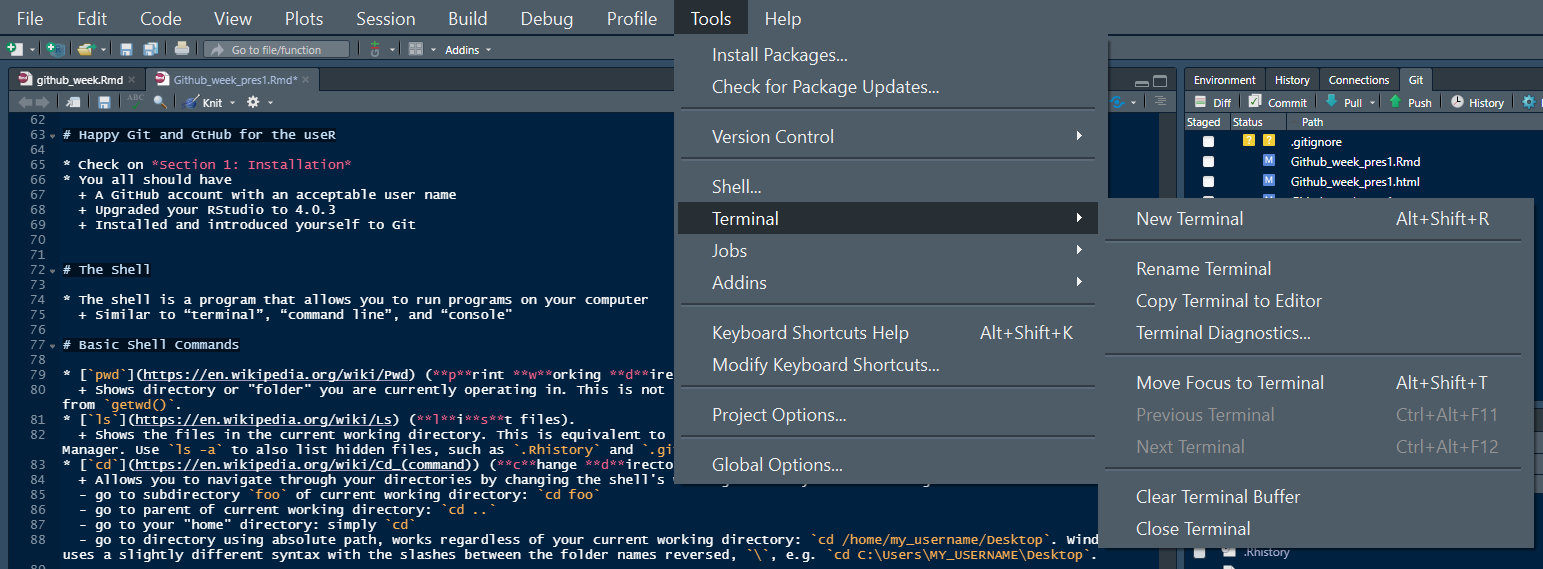
\includegraphics{pres_figs/terminal.png}

\end{frame}

\begin{frame}[fragile]{Basic Shell Commands}
\protect\hypertarget{basic-shell-commands}{}

\begin{itemize}
\tightlist
\item
  \href{https://en.wikipedia.org/wiki/Pwd}{\texttt{pwd}} (\textbf{p}rint
  \textbf{w}orking \textbf{d}irectory).

  \begin{itemize}
  \tightlist
  \item
    Shows directory or ``folder'' you are currently operating in.
  \end{itemize}
\item
  \href{https://en.wikipedia.org/wiki/Ls}{\texttt{ls}}
  (\textbf{l}i\textbf{s}t files).

  \begin{itemize}
  \tightlist
  \item
    Shows the files in the current working directory. This is equivalent
    to looking at the files in your Finder/Explorer/File Manager.
  \end{itemize}
\item
  \href{https://en.wikipedia.org/wiki/Cd_(command)}{\texttt{cd}}
  (\textbf{c}hange \textbf{d}irectory).

  \begin{itemize}
  \tightlist
  \item
    Allows you to navigate through your directories by changing the
    shell's working directory. You can navigate like so:
  \item
    go to subdirectory \texttt{foo} of current working directory:
    \texttt{cd\ foo}
  \item
    go to parent of current working directory: \texttt{cd\ ..}
  \item
    go to your ``home'' directory: simply \texttt{cd}
  \end{itemize}
\item
  Use arrow-up and arrow-down to repeat previous commands. Or search for
  previous commands with \texttt{CTRL} + \texttt{r}.
\end{itemize}

\end{frame}

\begin{frame}{Chapter 9: Connect to GitHub}
\protect\hypertarget{chapter-9-connect-to-github}{}

Objective: Make sure that you can all pull from and push to GitHub on
your local computer

\begin{itemize}
\tightlist
\item
  Order of operation

  \begin{enumerate}
  \tightlist
  \item
    Connect to GitHub
  \item
    Make a repository (or repo) on GitHub
  \item
    Clone the repo to your local computer (or remote)
  \item
    Make a local change, commit, and push
  \item
    Confirm local change propagated to the GitHub remote
  \item
    Clean up
  \end{enumerate}
\end{itemize}

\end{frame}

\begin{frame}{Connect to GitHub}
\protect\hypertarget{connect-to-github}{}

\begin{itemize}
\tightlist
\item
  Start by going to \url{https://github.com} and logging in
\end{itemize}

\begin{figure}
\centering
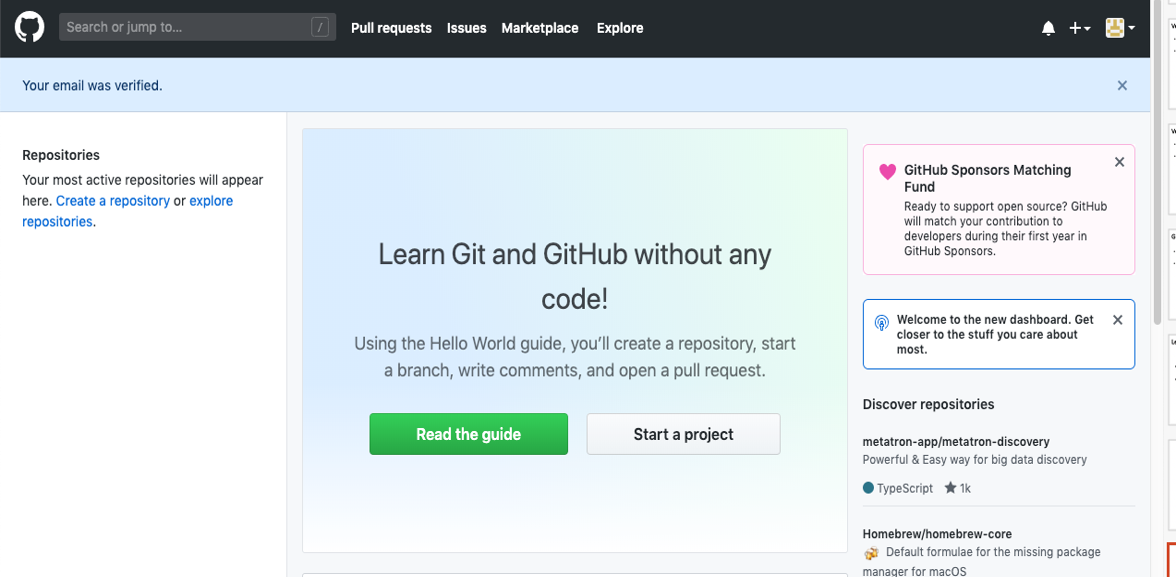
\includegraphics{pres_figs/homepage.png}
\caption{Homepage should look like this}
\end{figure}

\end{frame}

\begin{frame}{Make a repo on GitHub}
\protect\hypertarget{make-a-repo-on-github}{}

Click the plus, then the ``New repository'' button.

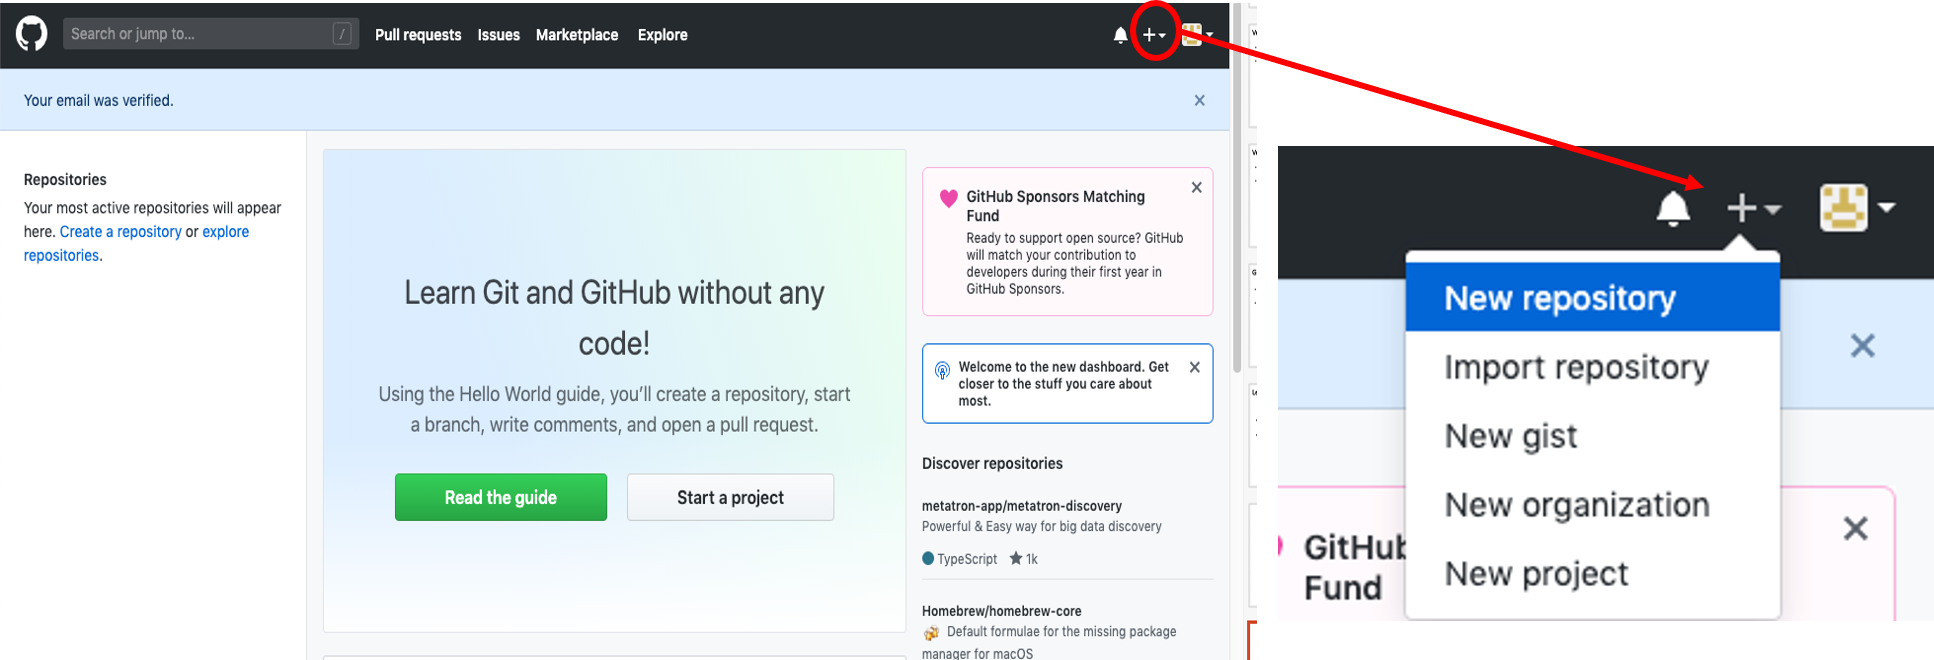
\includegraphics{pres_figs/new_repo.png}

\end{frame}

\begin{frame}[fragile]{Make a repo on GitHub}
\protect\hypertarget{make-a-repo-on-github-1}{}

\begin{columns}[T]
\begin{column}{0.48\textwidth}
\begin{itemize}
\tightlist
\item
  How to fill this in:

  \begin{itemize}
  \tightlist
  \item
    Repository name: \texttt{myrepo} (or whatever you wish, we'll delete
    this soon anyway).
  \item
    Description: ``testing my setup'' (or whatever, but some text is
    good for the README).
  \item
    Public.
  \item
    YES Initialize this repository with a README.
  \end{itemize}
\item
  For everything else, just accept the default.
\item
  Click big green button ``Create repository.''
\end{itemize}
\end{column}

\begin{column}{0.48\textwidth}
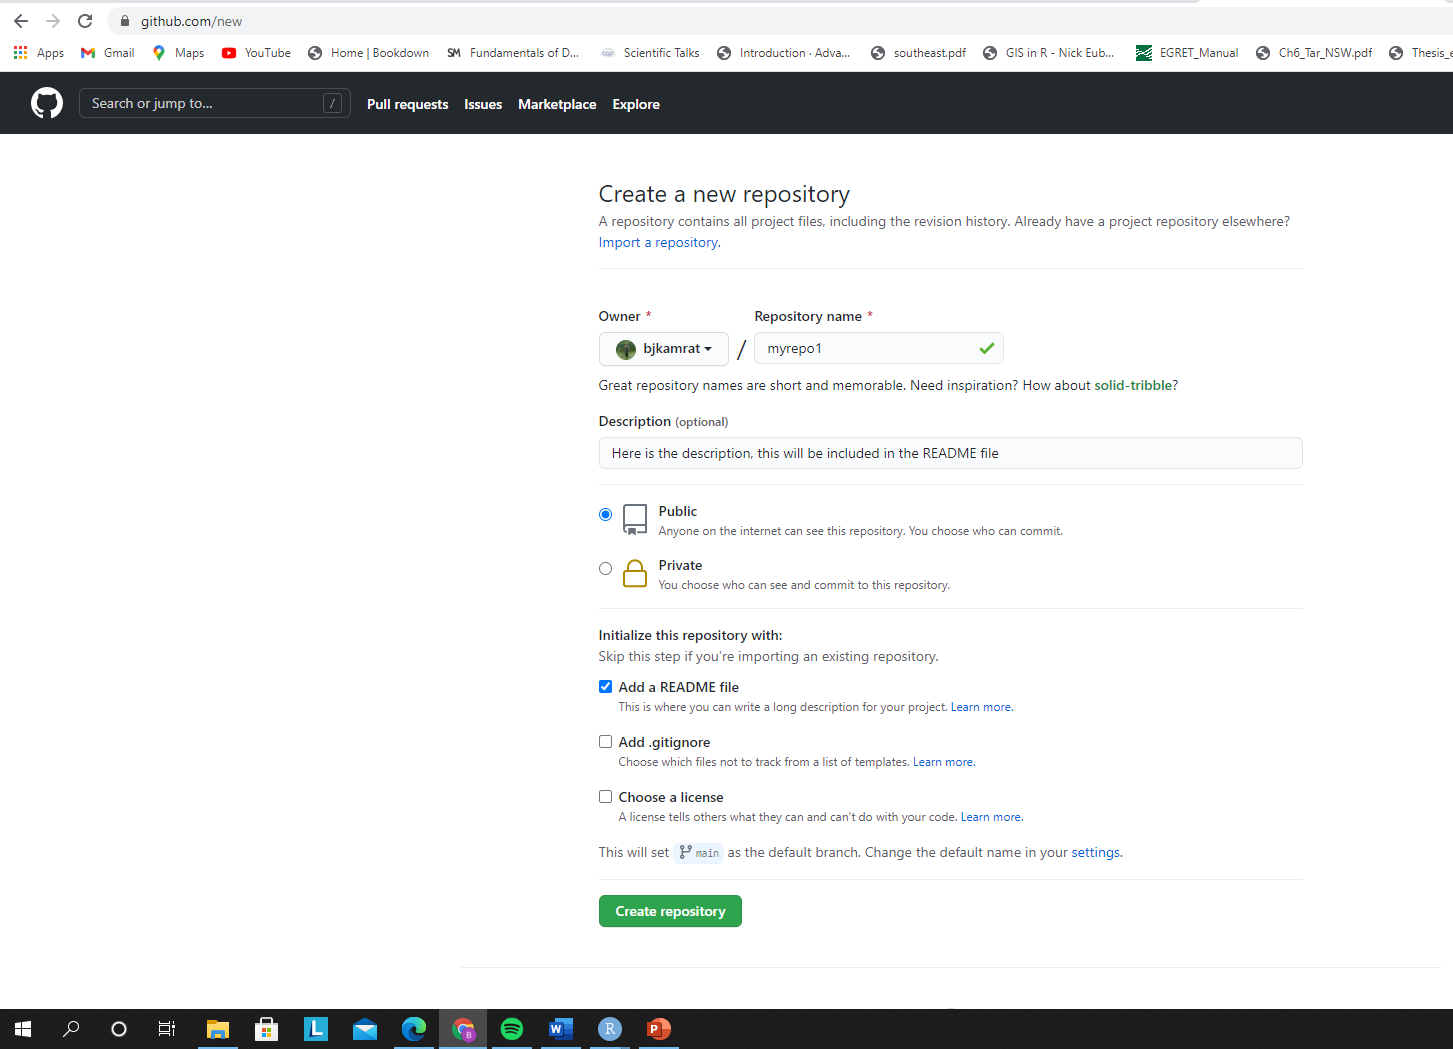
\includegraphics{pres_figs/new_repo_main.png}
\end{column}
\end{columns}

\end{frame}

\begin{frame}{Make a repo on GitHub}
\protect\hypertarget{make-a-repo-on-github-2}{}

\begin{figure}
\centering
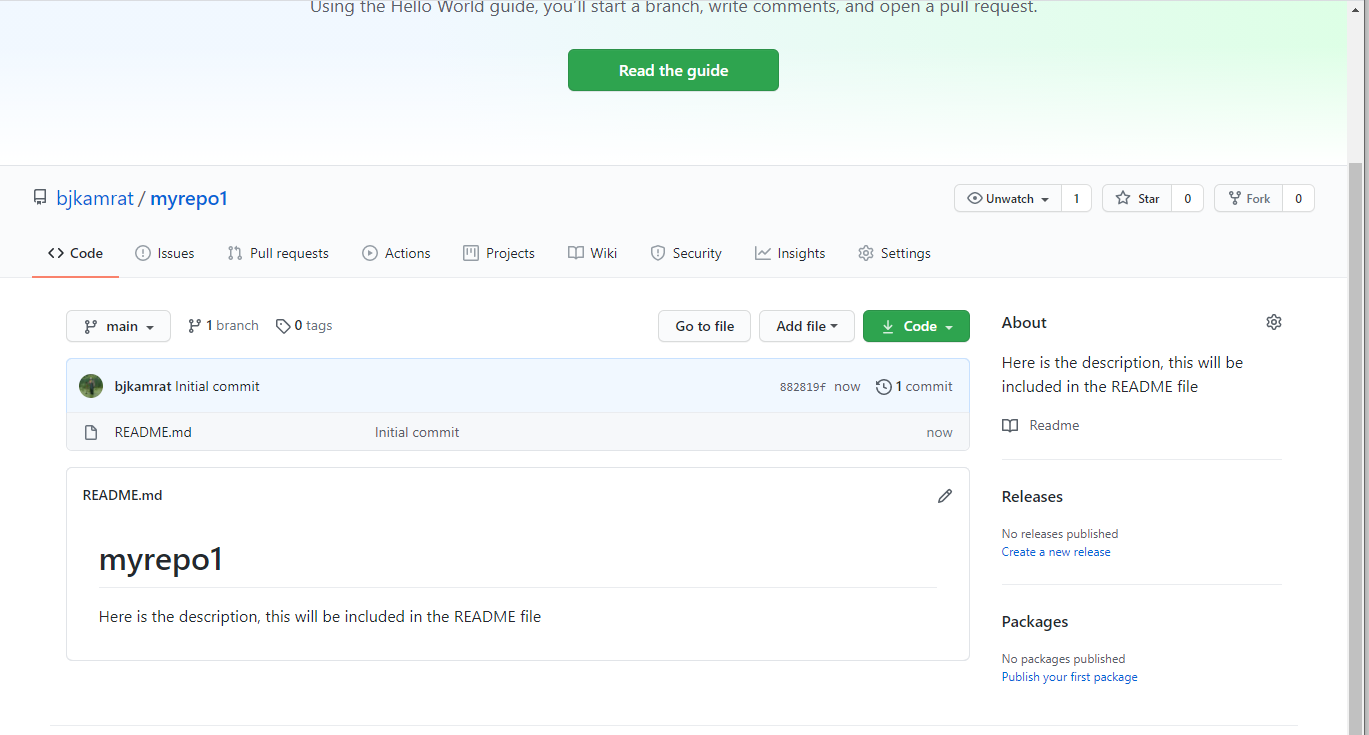
\includegraphics{pres_figs/new_repo_mainpage.png}
\caption{You should see this}
\end{figure}

\end{frame}

\begin{frame}{Clone the repo to your local computer}
\protect\hypertarget{clone-the-repo-to-your-local-computer}{}

Copy the HTTPS clone URL to your clipboard via the green ``Clone or
Download'' button.

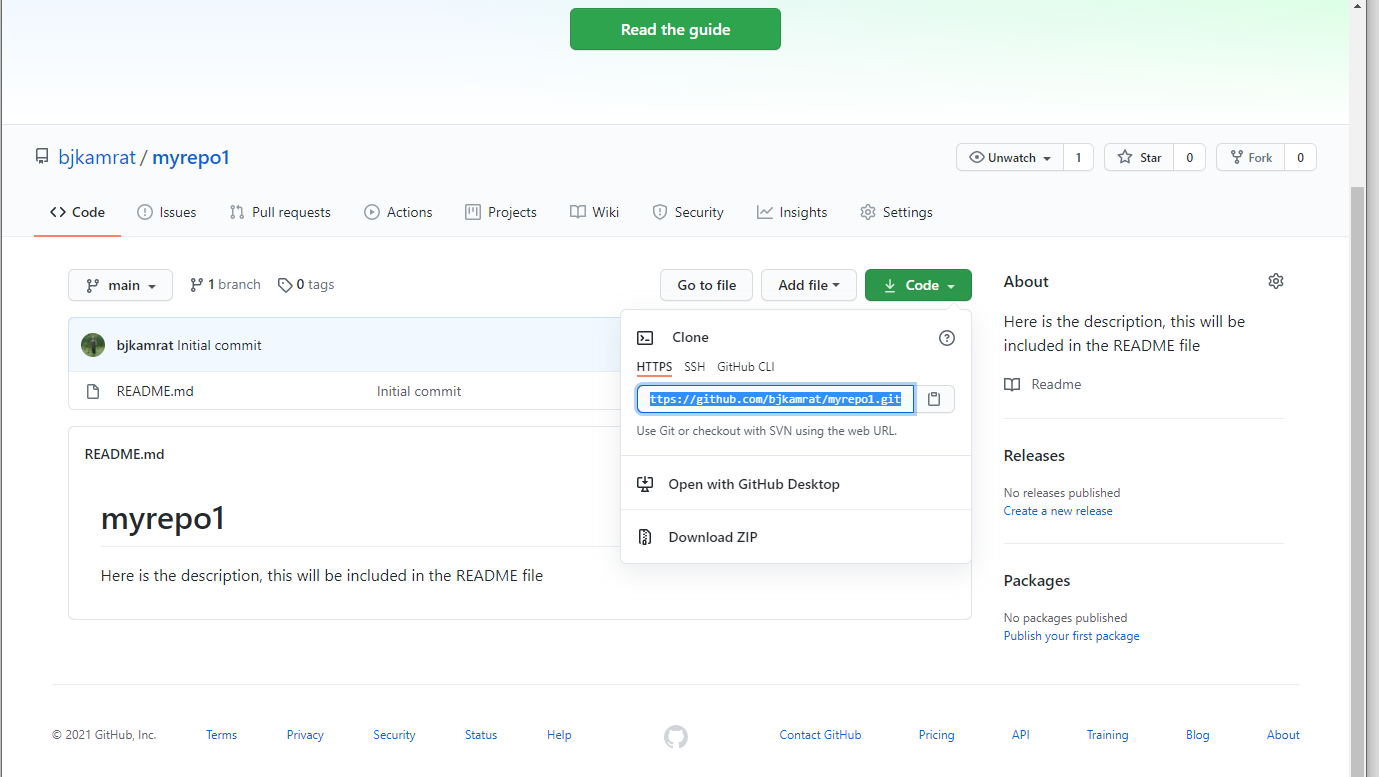
\includegraphics{pres_figs/clone.png}

\end{frame}

\begin{frame}[fragile]{Clone the repo to your local computer}
\protect\hypertarget{clone-the-repo-to-your-local-computer-1}{}

\begin{itemize}
\tightlist
\item
  Go to Tools \textgreater{} Terminal \textgreater{} New Terminal

  \begin{itemize}
  \tightlist
  \item
    Pay attention to the directory you're in!
  \item
    Use \texttt{pwd} to display the working directory, if not already
    displayed.
  \item
    Use \texttt{cd} to change directory.
  \end{itemize}
\item
  Clone \texttt{myrepo} from GitHub to your computer.

  \begin{itemize}
  \tightlist
  \item
    This URL should have \textbf{your GitHub username} and the name of
    \textbf{your practice repo}.
  \item
    Should be able to paste the copied HTTPS from Clone
  \end{itemize}
\end{itemize}

\begin{Shaded}
\begin{Highlighting}[]
\FunctionTok{git}\NormalTok{ clone https://github.com/YOUR-USERNAME/YOUR-REPOSITORY.git}
\end{Highlighting}
\end{Shaded}

\end{frame}

\begin{frame}[fragile]{Clone the repo to your local computer}
\protect\hypertarget{clone-the-repo-to-your-local-computer-2}{}

This should look something like this:

\begin{Shaded}
\begin{Highlighting}[]
\ExtensionTok{Cloning}\NormalTok{ into }\StringTok{'myrepo'}\NormalTok{...}
\ExtensionTok{remote}\NormalTok{: Enumerating objects: 3, done.}
\ExtensionTok{remote}\NormalTok{: Counting objects: 100% (3/3), }\KeywordTok{done}\ExtensionTok{.}
\ExtensionTok{remote}\NormalTok{: Compressing objects: 100% (2/2), }\KeywordTok{done}\ExtensionTok{.}
\ExtensionTok{remote}\NormalTok{: Total 3 (delta 0), }\ExtensionTok{reused}\NormalTok{ 0 (delta 0), }\ExtensionTok{pack-reused}\NormalTok{ 0}
\ExtensionTok{Receiving}\NormalTok{ objects: 100% (3/3), }\KeywordTok{done}\ExtensionTok{.}
\end{Highlighting}
\end{Shaded}

\end{frame}

\begin{frame}[fragile]{Clone the repo to your local computer}
\protect\hypertarget{clone-the-repo-to-your-local-computer-3}{}

\begin{itemize}
\tightlist
\item
  Make this new repo your working directory
\end{itemize}

\begin{Shaded}
\begin{Highlighting}[]
\NormalTok{$ }\BuiltInTok{cd}\NormalTok{ myrepo}
\end{Highlighting}
\end{Shaded}

\begin{itemize}
\tightlist
\item
  List its files
\end{itemize}

\begin{Shaded}
\begin{Highlighting}[]
\NormalTok{$ }\FunctionTok{ls} 
\ExtensionTok{README.md}
\end{Highlighting}
\end{Shaded}

\begin{itemize}
\tightlist
\item
  Display the README
\end{itemize}

\begin{Shaded}
\begin{Highlighting}[]
\NormalTok{$ }\FunctionTok{head}\NormalTok{ README.md}
\CommentTok{# myrepo}
\ExtensionTok{tutorial}\NormalTok{ devlopment}
\end{Highlighting}
\end{Shaded}

\end{frame}

\begin{frame}[fragile]{Clone the repo to your local computer}
\protect\hypertarget{clone-the-repo-to-your-local-computer-4}{}

\begin{itemize}
\tightlist
\item
  Now get some information on its connection to GitHub
\end{itemize}

\begin{Shaded}
\begin{Highlighting}[]
\FunctionTok{git}\NormalTok{ remote show origin}
\end{Highlighting}
\end{Shaded}

This should look something like this:

\begin{Shaded}
\begin{Highlighting}[]
\ExtensionTok{*}\NormalTok{ remote origin}
  \ExtensionTok{Fetch}\NormalTok{ URL: https://github.com/bjkamrat/myrepo1.git}
  \ExtensionTok{Push}\NormalTok{  URL: https://github.com/bjkamrat/myrepo1.git}
  \ExtensionTok{HEAD}\NormalTok{ branch: main}
  \ExtensionTok{Remote}\NormalTok{ branch:}
    \ExtensionTok{main}\NormalTok{ tracked}
  \ExtensionTok{Local}\NormalTok{ branch configured for }\StringTok{'git pull'}\NormalTok{:}
    \ExtensionTok{main}\NormalTok{ merges with remote main}
  \ExtensionTok{Local}\NormalTok{ ref configured for }\StringTok{'git push'}\NormalTok{:}
    \ExtensionTok{main}\NormalTok{ pushes to main (up to date)}
\end{Highlighting}
\end{Shaded}

\end{frame}

\begin{frame}[fragile]{Make a local change, commit, and push}
\protect\hypertarget{make-a-local-change-commit-and-push}{}

Add a line to README and verify that Git notices the change:

\begin{Shaded}
\begin{Highlighting}[]
\BuiltInTok{echo} \StringTok{"A line I wrote on my local computer"} \OperatorTok{>>}\NormalTok{ README.md}
\FunctionTok{git}\NormalTok{ status}
\end{Highlighting}
\end{Shaded}

This should look something like this:

\begin{Shaded}
\begin{Highlighting}[]
\ExtensionTok{On}\NormalTok{ branch main}
\ExtensionTok{Your}\NormalTok{ branch is up to date with }\StringTok{'origin/main'}\NormalTok{.}

\ExtensionTok{Changes}\NormalTok{ not staged for commit:}
  \KeywordTok{(}\ExtensionTok{use} \StringTok{"git add <file>..."}\NormalTok{ to update what will be committed}\KeywordTok{)}
  \KeywordTok{(}\ExtensionTok{use} \StringTok{"git restore <file>..."}\NormalTok{ to discard changes in working directory}\KeywordTok{)}
        \ExtensionTok{modified}\NormalTok{:   README.md}

\ExtensionTok{no}\NormalTok{ changes added to commit (use }\StringTok{"git add"}\NormalTok{ and/or }\StringTok{"git commit -a"}\NormalTok{)}
\end{Highlighting}
\end{Shaded}

\end{frame}

\begin{frame}[fragile]{Make a local change, commit, and push}
\protect\hypertarget{make-a-local-change-commit-and-push-1}{}

\begin{columns}[T]
\begin{column}{0.48\textwidth}
\begin{itemize}
\tightlist
\item
  Stage (``add'') and commit this change
\item
  Push to your remote repo on GitHub.

  \begin{itemize}
  \tightlist
  \item
    \emph{If you're a new GitHub user, you will be challenged for your
    GitHub username and password. Provide them!}
  \end{itemize}
\end{itemize}

\begin{Shaded}
\begin{Highlighting}[]
\FunctionTok{git}\NormalTok{ add -A}
\FunctionTok{git}\NormalTok{ commit -m }\StringTok{"A commit from my local computer"}
\FunctionTok{git}\NormalTok{ push}
\end{Highlighting}
\end{Shaded}

Note: \texttt{-m\ "blah\ blah\ blah"} piece is very important + It adds
the required commit message to the commit
\end{column}

\begin{column}{0.48\textwidth}
This should look something like this:

\begin{Shaded}
\begin{Highlighting}[]
\NormalTok{$ }\FunctionTok{git}\NormalTok{ add -A}
\ExtensionTok{warning}\NormalTok{: LF will be replaced by CRLF in README.md.}
\ExtensionTok{The}\NormalTok{ file will have its original line endings in your working directory}

\NormalTok{$ }\FunctionTok{git}\NormalTok{ commit -m }\StringTok{"A commit from my local computer"}
\NormalTok{[}\ExtensionTok{main}\NormalTok{ be70f46] A commit from my local computer}
 \ExtensionTok{1}\NormalTok{ file changed, 1 insertion(+)}
 
\NormalTok{$ }\FunctionTok{git}\NormalTok{ push}
\ExtensionTok{Enumerating}\NormalTok{ objects: 5, done.}
\ExtensionTok{Counting}\NormalTok{ objects: 100% (5/5), }\KeywordTok{done}\ExtensionTok{.}
\ExtensionTok{Delta}\NormalTok{ compression using up to 8 threads}
\ExtensionTok{Compressing}\NormalTok{ objects: 100% (2/2), }\KeywordTok{done}\ExtensionTok{.}
\ExtensionTok{Writing}\NormalTok{ objects: 100% (3/3), }\ExtensionTok{346}\NormalTok{ bytes }\KeywordTok{|} \ExtensionTok{346.00}\NormalTok{ KiB/s, done.}
\ExtensionTok{Total}\NormalTok{ 3 (delta 0), }\ExtensionTok{reused}\NormalTok{ 0 (delta 0), }\ExtensionTok{pack-reused}\NormalTok{ 0}
\ExtensionTok{To}\NormalTok{ https://github.com/bjkamrat/myrepo1.git}
   \ExtensionTok{882819f..be70f46}\NormalTok{  main -}\OperatorTok{>}\NormalTok{ main}
\end{Highlighting}
\end{Shaded}
\end{column}
\end{columns}

\end{frame}

\begin{frame}{Confirm local change propgated to GitHub}
\protect\hypertarget{confirm-local-change-propgated-to-github}{}

\begin{enumerate}
\item
  Go back to the browser. I assume we're still viewing your new GitHub
  repo.
\item
  Refresh.
\item
  You should see the new ``A line I wrote on my local computer'' in the
  README.
\item
  If you click on ``commits,'' you should see one with the message ``A
  commit from my local computer.''
\end{enumerate}

\end{frame}

\begin{frame}[fragile]{Clean up}
\protect\hypertarget{clean-up}{}

\textbf{Local} When you're ready to clean up, you can delete the local
repo any way you like. It's just a regular directory on your computer.

Here's how to do that in the shell, if current working directory is
\texttt{myrepo}:

\begin{Shaded}
\begin{Highlighting}[]
\BuiltInTok{cd}\NormalTok{ ..}
\FunctionTok{rm}\NormalTok{ -rf myrepo/}
\end{Highlighting}
\end{Shaded}

\textbf{GitHub} In the browser, go to your repo's landing page on
GitHub. Click on ``Settings''.

Scroll down, click on ``delete repository,'' and do as it asks.

\end{frame}

\begin{frame}{Now, lets use GitHub and RStudio together (Chapter 15)}
\protect\hypertarget{now-lets-use-github-and-rstudio-together-chapter-15}{}

\begin{itemize}
\tightlist
\item
  This workflow will be similar to the previous section
\item
  More like what you will be doing in the future by using Git within
  RStudio
\end{itemize}

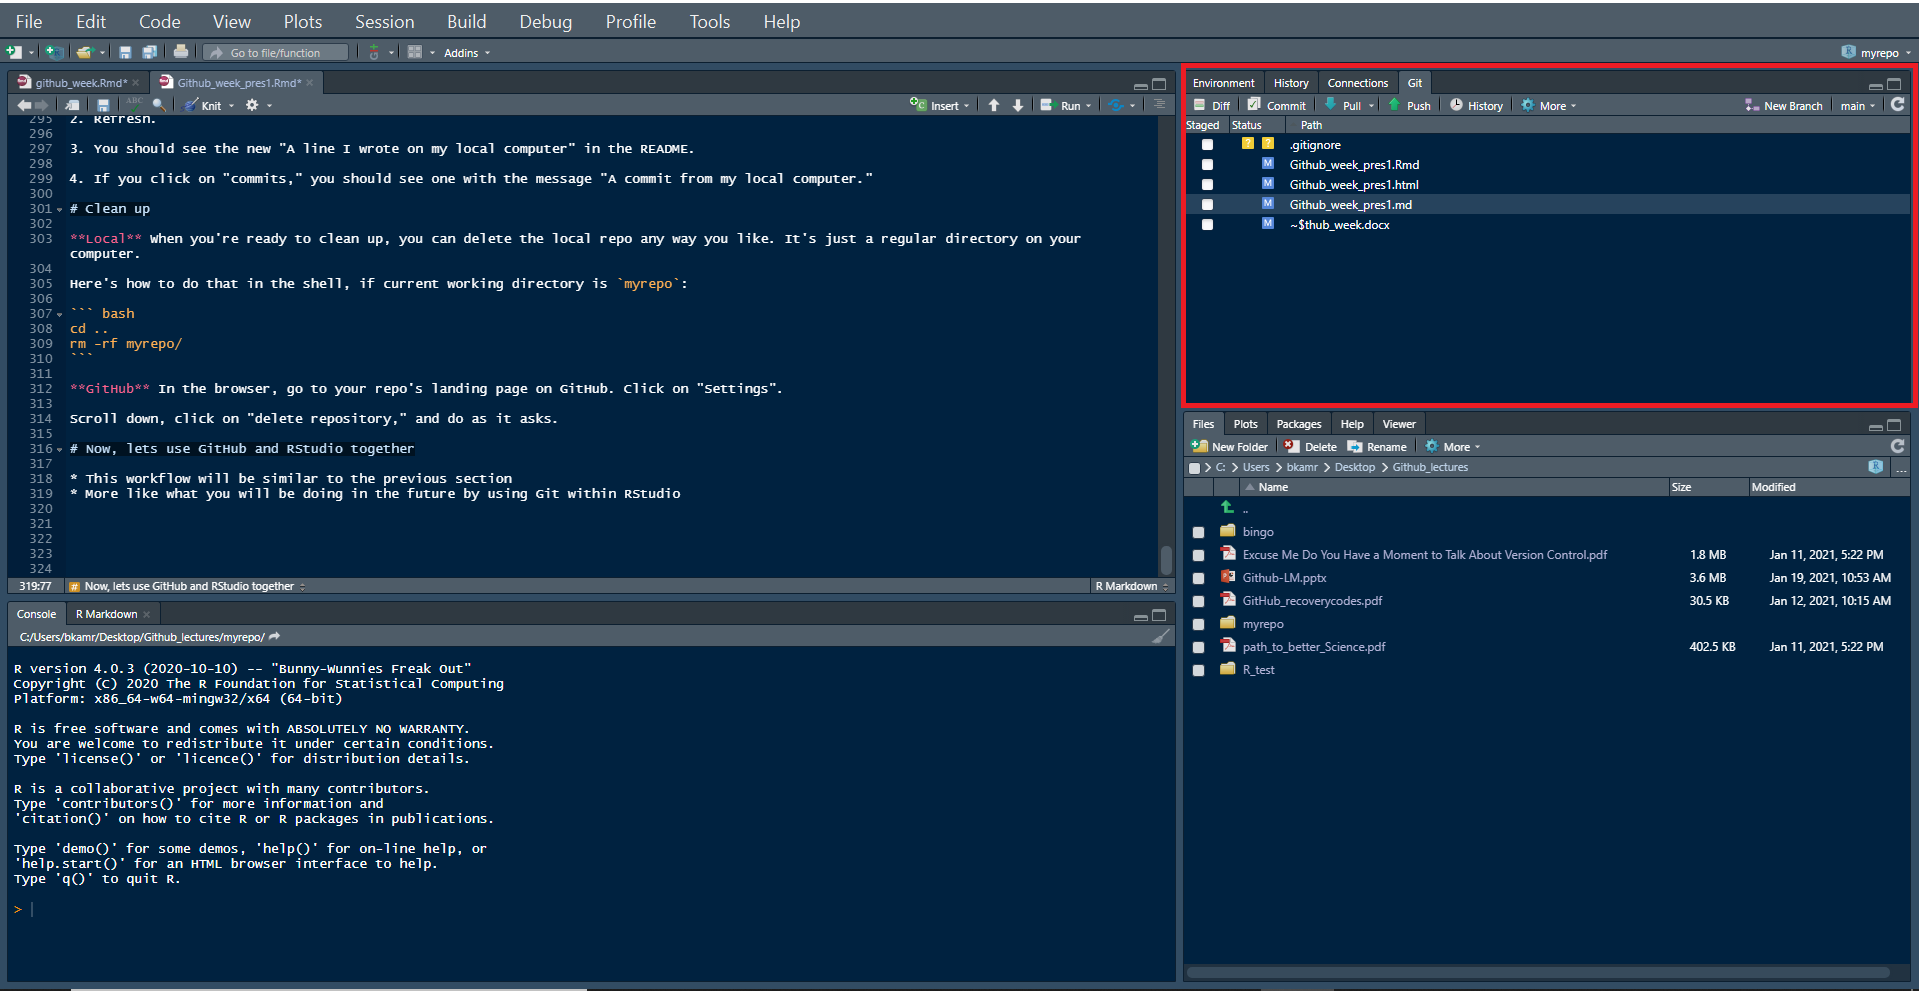
\includegraphics{pres_figs/git_in_rstuido.png}

\end{frame}

\begin{frame}[fragile]{Start by making a repo in GitHub}
\protect\hypertarget{start-by-making-a-repo-in-github}{}

\begin{itemize}
\tightlist
\item
  This will be done using the same exact method as before
\item
  Remember

  \begin{itemize}
  \tightlist
  \item
    Repository name: \texttt{myrepo} (or whatever you wish, we'll delete
    this soon anyway).
  \item
    Description: ``testing my setup'' (or whatever, but some text is
    good for the README).
  \item
    Public.
  \item
    YES Initialize this repository with a README.
  \end{itemize}
\item
  For everything else, just accept the default.
\item
  Click big green button ``Create repository.''
\end{itemize}

\end{frame}

\begin{frame}[fragile]{New RStudio Project via git clone}
\protect\hypertarget{new-rstudio-project-via-git-clone}{}

\begin{columns}[T]
\begin{column}{0.48\textwidth}
\begin{itemize}
\tightlist
\item
  Start a new Project in RStudio

  \begin{itemize}
  \tightlist
  \item
    \emph{File \textgreater{} New Project \textgreater{} Version Control
    \textgreater{} Git}.
  \item
    In the ``repository URL'' paste the URL of your new GitHub
    repository.

    \begin{itemize}
    \tightlist
    \item
      \texttt{https://github.com/bjkamrat/myrepo.git}
    \end{itemize}
  \end{itemize}
\item
  Be intentional about where you create this Project.
\item
  Suggest you ``Open in new session''.
\item
  Click ``Create Project'' to create a new directory, which will be:

  \begin{itemize}
  \tightlist
  \item
    a directory or ``folder'' on your computer
  \item
    a Git repository, linked to a remote GitHub repository
  \item
    an RStudio Project
  \end{itemize}
\end{itemize}
\end{column}

\begin{column}{0.48\textwidth}
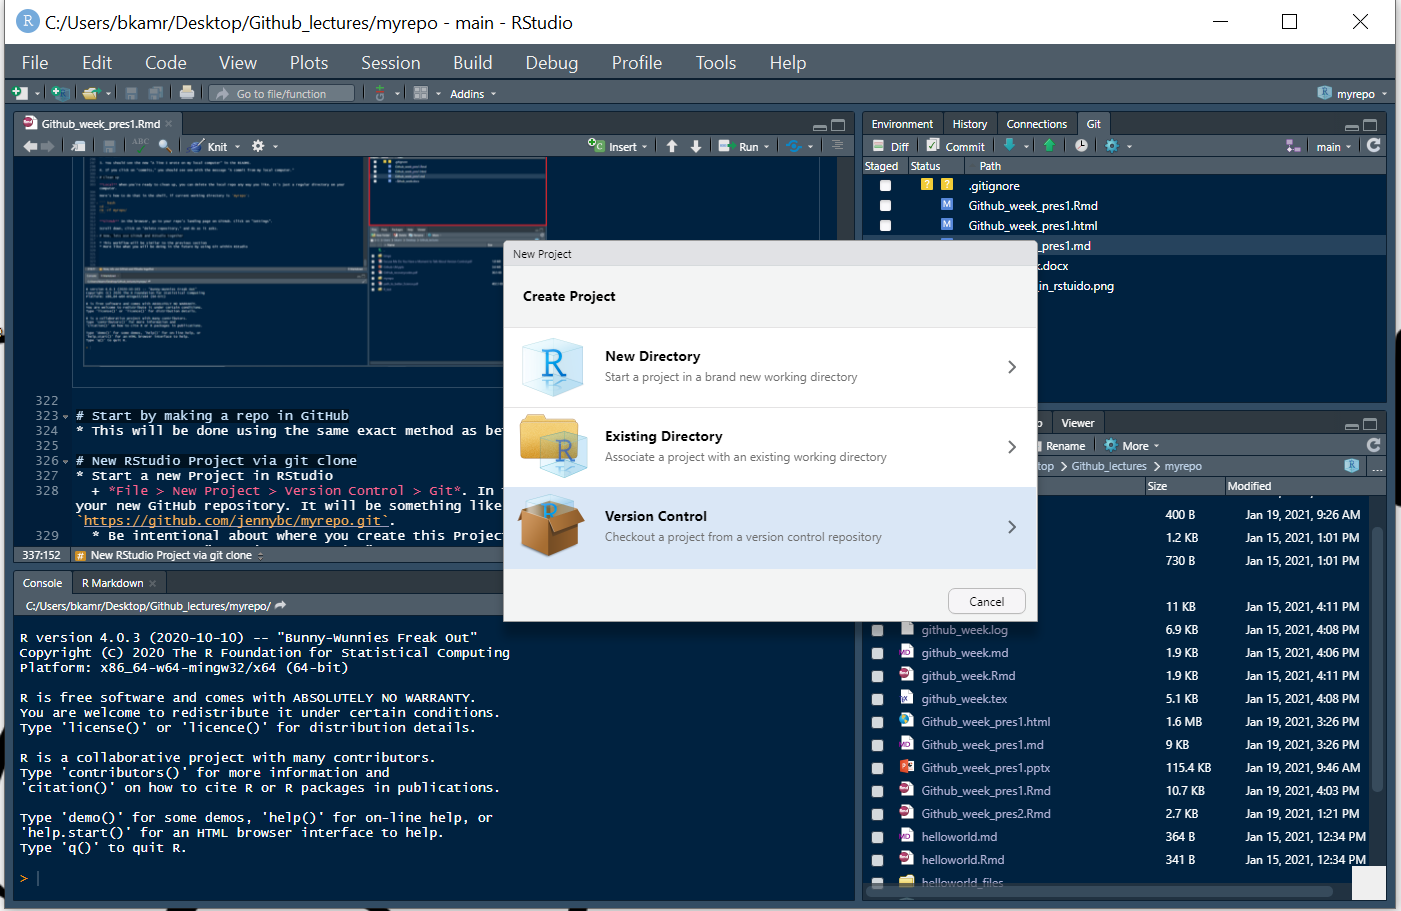
\includegraphics{pres_figs/new_project_rstudio.png}
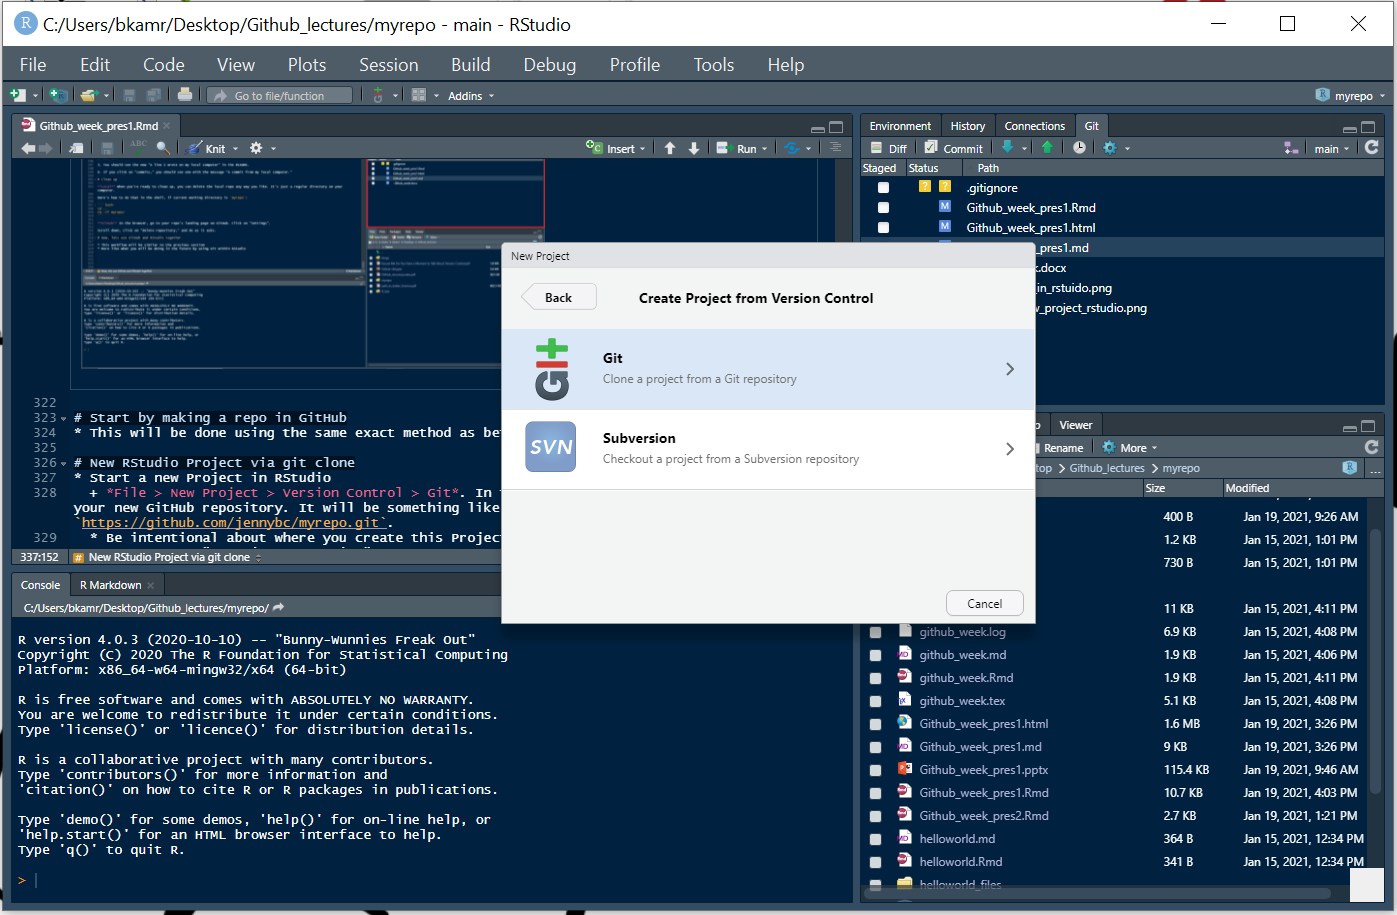
\includegraphics{pres_figs/new_project_rstudio_git.png}
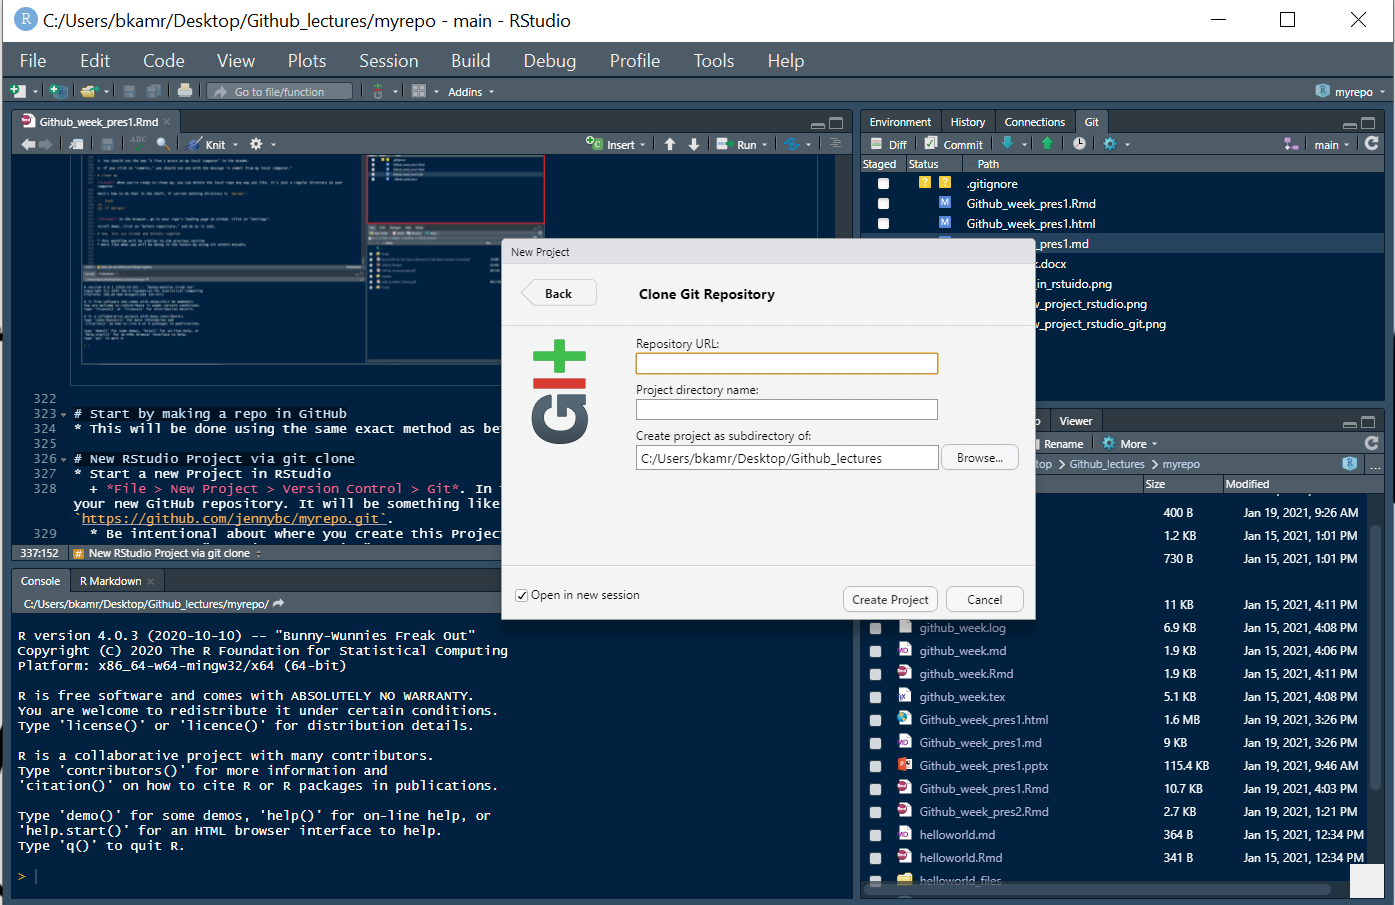
\includegraphics{pres_figs/new_project_rstudio_git_url.png}
\end{column}
\end{columns}

\begin{itemize}
\tightlist
\item
  \textbf{All of your R projects should have this set-up.}
\end{itemize}

\end{frame}

\begin{frame}[fragile]{New RStudio Project via git clone}
\protect\hypertarget{new-rstudio-project-via-git-clone-1}{}

\begin{itemize}
\tightlist
\item
  The \texttt{README.md} file that we created on GitHub in the previous
  step should be there.

  \begin{itemize}
  \tightlist
  \item
    Look in RStudio's file browser pane for the \texttt{README.md} file.
  \end{itemize}
\item
  There's a big advantage to the ``GitHub first, then RStudio'' workflow

  \begin{itemize}
  \tightlist
  \item
    The remote GitHub repo is added as a remote for your local repo and
    your local \texttt{master} branch is now tracking \texttt{master} on
    GitHub.
  \item
    This is a technical but it means that you are now set up to push and
    pull.
  \end{itemize}
\end{itemize}

\end{frame}

\begin{frame}[fragile]{Make local changes, save, commit}
\protect\hypertarget{make-local-changes-save-commit}{}

\textbf{Do this every time you finish a valuable chunk of work, probably
many times a day.}

\begin{itemize}
\item
  In RStudio, open and modify the \texttt{README.md} file, by adding the
  line ``This is a line from RStudio''. Save your changes.
\item
  Commit these changes to your local repo.

  \begin{enumerate}
  \tightlist
  \item
    Click the ``Git'' tab in upper right pane (Note:
    Environment\textbar{}History\textbar{}Connections\textbar{}Git)
  \item
    Check ``Staged'' box for any files whose existence or modifications
    you want to commit.
  \end{enumerate}

  \begin{itemize}
  \tightlist
  \item
    click on ``Diff'' for a Git pop-up of changes made
  \end{itemize}

  \begin{enumerate}
  \setcounter{enumi}{2}
  \tightlist
  \item
    If you're not already in the Git pop-up, click ``Commit''
  \item
    Type a message in ``Commit message'', such as ``Commit from
    RStudio''.
  \item
    Click ``Commit''
  \end{enumerate}
\end{itemize}

\end{frame}

\begin{frame}[fragile]{Push your local changes to GitHub}
\protect\hypertarget{push-your-local-changes-to-github}{}

\textbf{Do this a few times a day, but possibly less often than you
commit.}

\begin{itemize}
\tightlist
\item
  At this point your changes have been made at the local level, but not
  pushed online yet.
\end{itemize}

What do we need to do? 1. let's stop and pull from GitHub. + Click the
blue ``Pull'' button. + You should get the message ``Already
up-to-date.'' + Why? + Establish this habit + If you make changes to the
repo in the browser or from another machine or (one day) a collaborator
has pushed, you will be happier if you pull those changes in before you
attempt to push.

\begin{enumerate}
\setcounter{enumi}{1}
\tightlist
\item
  Push your local changes to GitHub
\end{enumerate}

\begin{itemize}
\tightlist
\item
  Click the green ``Push'' button\\
\item
  You should see some message along these lines.
\end{itemize}

\begin{Shaded}
\begin{Highlighting}[]
\NormalTok{[}\ExtensionTok{master}\NormalTok{ dc671f0] blah}
 \ExtensionTok{3}\NormalTok{ files changed, 22 insertions(+)}
 \ExtensionTok{create}\NormalTok{ mode 100644 .gitignore}
 \ExtensionTok{create}\NormalTok{ mode 100644 myrepo.Rproj}
\end{Highlighting}
\end{Shaded}

You have now pushed a change on you local computer to GitHub!

\end{frame}

\begin{frame}{Confirm the local change propagated to the GitHub remote}
\protect\hypertarget{confirm-the-local-change-propagated-to-the-github-remote}{}

\begin{itemize}
\tightlist
\item
  Go back to the browser. I assume we're still viewing your new GitHub
  repo.
\item
  Refresh.
\item
  You should see the new ``This is a line from RStudio'' in the README.

  \begin{itemize}
  \tightlist
  \item
    If you click on ``commits,'' you should see one with the message
    ``Commit from RStudio''.
  \end{itemize}
\end{itemize}

\end{frame}

\begin{frame}{Make a change on GitHub}
\protect\hypertarget{make-a-change-on-github}{}

\begin{enumerate}
\tightlist
\item
  Click on README.md in the file listing on GitHub.
\end{enumerate}

\begin{itemize}
\tightlist
\item
  In the upper right corner, click on the pencil for ``Edit this file''.
\end{itemize}

\begin{enumerate}
\setcounter{enumi}{1}
\tightlist
\item
  Add a line to this file, such as ``Line added from GitHub.''
\item
  Edit the commit message in ``Commit changes'' or accept the default.
\item
  Click the big green button ``Commit changes.''
\end{enumerate}

\end{frame}

\begin{frame}{Now, Pull the updated repo from GitHub to local computer}
\protect\hypertarget{now-pull-the-updated-repo-from-github-to-local-computer}{}

So, Back in RStudio

\begin{enumerate}
\tightlist
\item
  Inspect your README.md.
\end{enumerate}

\begin{itemize}
\tightlist
\item
  It should NOT have the line ``Line added from GitHub''. It should be
  as you left it.
\end{itemize}

\begin{enumerate}
\setcounter{enumi}{1}
\tightlist
\item
  Click the blue Pull button.
\end{enumerate}

\begin{itemize}
\tightlist
\item
  Look at README.md again. You should now see the new line there.
\end{itemize}

\end{frame}

\begin{frame}{For the future}
\protect\hypertarget{for-the-future}{}

Now just \ldots{} repeat. Do work somewhere. Commit it. Push it or pull
it* depending on where you did it, but get local and remote ``synced
up''. Repeat.

* Note that in general (and especially in future when collaborating with
other developers) you will usually need to pull changes from the remote
(GitHub) before pushing the local changes you have made. For this
reason, it's a good idea to try and get into the habit of pulling before
you attempt to push.

\end{frame}

\begin{frame}{Coursework for this week}
\protect\hypertarget{coursework-for-this-week}{}

With the rest of the class period, I would like you to begin working
through chapters 16, 17, and 18 from happygitwithr.com

For Thursday (2/4/21), you need to

\begin{itemize}
\tightlist
\item
  Complete chapters 16, 17, and 18
\item
  Finish reading Byran article (Excuse Me\ldots{})
\end{itemize}

On Thursday, we will

\begin{itemize}
\tightlist
\item
  Go over any questions
\item
  Get more into GitHub basics
\item
  Work through some additional material
\item
  Then begin an exercise due next Tuesday (2/9/21)
\end{itemize}

\end{frame}

\end{document}
